
\documentclass{beamer}
 
\usepackage[utf8]{inputenc}
\usepackage{mathtools}
\usepackage{tikz}
\usetikzlibrary{calc}

\usetheme{CambridgeUS}
\useoutertheme{split}
\setbeamertemplate{title page}[default][colsep=-4bp,rounded=true]
 
%Information to be included in the title page:
\title{Semantic Security}
\author{Rohit Musti}
\institute{CUNY - Hunter College}
\date{\today}
 
\begin{document}
 
\frame{\titlepage}
\begin{frame}
    \frametitle{One Time Pad Security Game: Semantic Security}
    \begin{tikzpicture}
      \pause
        \node[draw] (Adversary) at (-3, 2) {\(\mathcal{A}\)}; 
        \draw[thick] (Adversary) -- ++(0, -4); 
        \draw[thick] (Adversary) -- ++(-2, 0);
        \draw[thick] (-3, -2) -- ++(-2, 0);

      \pause
        \node[draw] (Challenger) at (3,2) {\(\mathcal{C}\)}; 
        \draw[thick] (Challenger) -- ++(0, -4);
        \draw[thick] (Challenger) -- ++(2, 0);
        \draw[thick] (3, -2) -- ++(2, 0);

      \pause
        \node[draw=none,fill=none,anchor=east, font=\footnotesize] (choice0) at ($(Adversary) + (0,-.75)$) {\(m_0, m_1 \xleftarrow[]{R} \mathcal{M}\)};
      \pause
        \draw[->,thick] ($(Adversary)+(0,-1)$) -- ($(Challenger)+(0,-1)$) node [pos=0.5,above,font=\footnotesize] {\(m_0, m_1\)};
      \pause
        \node[draw=none,fill=none,anchor=west, font=\footnotesize] (bit) at ($(Challenger) + (0,-1.45)$) {\(b \xleftarrow[]{R} \{0, 1\}, k \xleftarrow[]{R} K \)};
      \pause
        \node[draw=none,fill=none,anchor=west, font=\footnotesize] (bit) at ($(Challenger) + (0,-2.05)$) {\(E(k, m_b) = c\)};
      \pause
        \draw[->,thick] ($(Challenger)+(0,-2.5)$) -- ($(Adversary)+(0,-2.5)$) node [pos=0.5,above,font=\footnotesize] {\(c \)};
      \pause
        \draw[->,thick] ($(Adversary)+(-1,-4)$) -- ($(Adversary)+(-1,-5)$) node [pos=0.5,left,font=\footnotesize] {\(b\)};
      \end{tikzpicture}
\end{frame}
\begin{frame}
    \frametitle{Semantic Security: Message Recovery Game}
    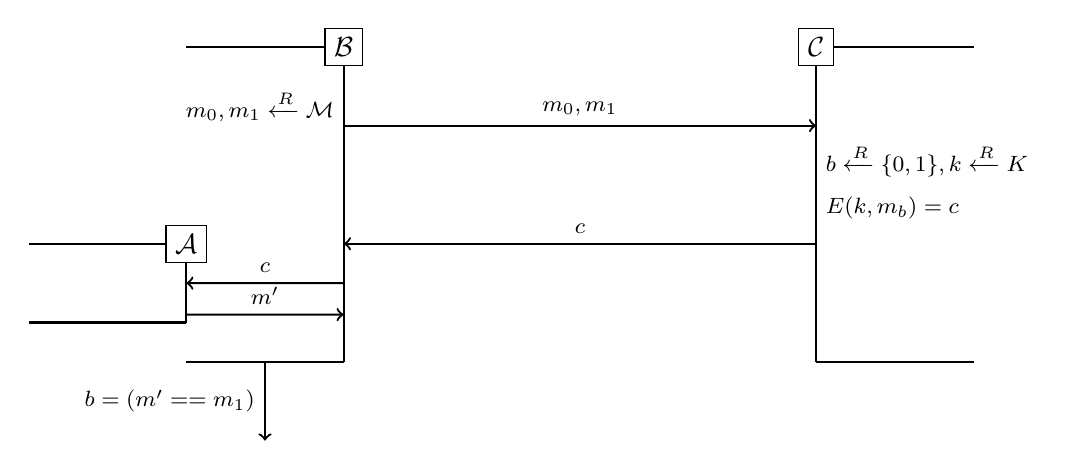
\begin{tikzpicture}


      \pause
        \node[draw] (Adversary) at (-3, 2) {\(\mathcal{B}\)}; 
        \draw[thick] (Adversary) -- ++(0, -4); 
        \draw[thick] (Adversary) -- ++(-2, 0);
        \draw[thick] (-3, -2) -- ++(-2, 0);

      \pause
        \node[draw] (Adversary2) at (-5, -0.5) {\(\mathcal{A}\)}; 
        \draw[thick] (Adversary2) -- ++(0, -1); 
        \draw[thick] (Adversary2) -- ++(-2, 0);
        \draw[thick] (-5, -1.5) -- ++(-2, 0);

      \pause
        \node[draw] (Challenger) at (3,2) {\(\mathcal{C}\)}; 
        \draw[thick] (Challenger) -- ++(0, -4);
        \draw[thick] (Challenger) -- ++(2, 0);
        \draw[thick] (3, -2) -- ++(2, 0);

      \pause
        \node[draw=none,fill=none,anchor=east, font=\footnotesize] (choice0) at ($(Adversary) + (0,-.75)$) {\(m_0, m_1 \xleftarrow[]{R} \mathcal{M}\)};
      \pause
        \draw[->,thick] ($(Adversary)+(0,-1)$) -- ($(Challenger)+(0,-1)$) node [pos=0.5,above,font=\footnotesize] {\(m_0, m_1\)};
      \pause
        \node[draw=none,fill=none,anchor=west, font=\footnotesize] (bit) at ($(Challenger) + (0,-1.45)$) {\(b \xleftarrow[]{R} \{0, 1\}, k \xleftarrow[]{R} K \)};
      \pause
        \node[draw=none,fill=none,anchor=west, font=\footnotesize] (bit) at ($(Challenger) + (0,-2.05)$) {\(E(k, m_b) = c\)};
      \pause
        \draw[->,thick] ($(Challenger)+(0,-2.5)$) -- ($(Adversary)+(0,-2.5)$) node [pos=0.5,above,font=\footnotesize] {\(c \)};

      \pause
        \draw[->,thick] ($(Adversary)+(0,-3)$) -- ($(Adversary2)+(0,-.5)$) node [pos=0.5,above,font=\footnotesize] {\(c \)};
      \pause
        \draw[->,thick] ($(Adversary2)+(0,-.9)$) -- ($(Adversary)+(0,-3.4)$) node [pos=0.5,above,font=\footnotesize] {\(m' \)};

      \pause
        \draw[->,thick] ($(Adversary)+(-1,-4)$) -- ($(Adversary)+(-1,-5)$) node [pos=0.5,left,font=\footnotesize] {\(b = (m' == m_1)\)};
      \end{tikzpicture}
\end{frame}
\end{document}
